\documentclass[10pt,letterpaper]{article}
\usepackage[utf8]{inputenc}
\usepackage{amsmath}
\usepackage{amsfonts}
\usepackage{amssymb}
\usepackage{graphicx}
\usepackage{etoolbox}
\usepackage{xcolor}
\usepackage{listings}
\usepackage{color}
\usepackage{subcaption}

\title{RBE 595 Motion Planning \\ \large Homework 2}
\author{Daniel Miller}

\renewcommand{\thesection}{}
\renewcommand{\thesubsection}{}

\setlength{\parskip}{\baselineskip}%
\setlength{\parindent}{0pt}%

\newcommand{\highlight}[1]{\colorbox{yellow}{$\displaystyle #1$}}

\begin{document}
\maketitle

\section{Problem 3.2}
\textbf{Question: } For distinct values of yaw, pitch, and roll, it is possible to generate the same rotation. In other words,  $ R(\alpha,\beta,\gamma) =
R(\alpha',\beta',\gamma')$ for some cases in which at least  $ \alpha
\not = \alpha$,  $ \beta \not = \beta'$, or $ \gamma \not = \gamma'$. Characterize the sets of angles for which this occurs.

\textbf{Answer: } Any single-axis rotation which aligns two of the rotation axes (i.e. Pitch up $\pi/2$ aligns global yaw with local roll). This "collapses" the rotation matrix to have a column with no angle variables in it, such as the one shown below. Effectively, this prevents the representation of any other roll, from this point. 

See this example from Wikipedia, which describes the above example (Pitch up: $\beta = \pi/2$)
\begin{align*}
R &= \begin{bmatrix}
1 & 0 & 0 \\
0 & \cos \alpha & -\sin \alpha \\
0 & \sin \alpha & \cos \alpha \end{bmatrix} \begin{bmatrix}
\cos \beta & 0 & \sin \beta \\
0 & 1 & 0 \\
-\sin \beta & 0 & \cos \beta \end{bmatrix} \begin{bmatrix}
\cos \gamma & -\sin \gamma & 0 \\
\sin \gamma & \cos \gamma & 0 \\
0 & 0 & 1 
\end{bmatrix} \\
R &= \begin{bmatrix}
1 & 0 & 0 \\
0 & \cos \alpha & -\sin \alpha \\
0 & \sin \alpha & \cos \alpha \end{bmatrix} \begin{bmatrix}
0 & 0 & 1 \\
0 & 1 & 0 \\
-1 & 0 & 0 \end{bmatrix} \begin{bmatrix}
\cos \gamma & -\sin \gamma & 0 \\
\sin \gamma & \cos \gamma & 0 \\
0 & 0 & 1 
\end{bmatrix} \\
R &= \begin{bmatrix}
0 & 0 & 1 \\
\sin ( \alpha + \gamma ) & \cos (\alpha + \gamma) & 0 \\
-\cos ( \alpha + \gamma ) & \sin (\alpha + \gamma) & 0 
\end{bmatrix} 
\end{align*}

As shown in the final matrix, $\alpha$ and $\gamma$ have "collapsed", and no longer allow for changes in each column of the matrix. Rotations about $\alpha$ or about $\gamma$ will produce identical results. 



\section{Problem 3.3}
\textbf{Question: } Using rotation matrices, prove that 2D rotation is commutative but 3D rotation is not.

\textbf{Answer: } 2D rotation is commutative, because the two angles, $\theta_1$ and $\theta_2$ rotate about the same axis, as shown here. 
\begin{align*}
R(\theta_1)R(\theta_2) &= \begin{bmatrix}
\cos \theta_1 & -\sin \theta_1 \\
\sin \theta_1 & \cos \theta_1
\end{bmatrix} \begin{bmatrix}
\cos \theta_2 & -\sin \theta_2 \\
\sin \theta_2 & \cos \theta_2
\end{bmatrix} \\
&= \begin{bmatrix}
C_1C_2 - S_1S_2 & -C_1S_2 - S_1C_2 \\
S_1C_2 + C_1S_2 & -S_1S_2 + C_1C_2
\end{bmatrix} = \begin{bmatrix}
\cos \theta_{12} & -\sin \theta_{12} \\
\sin \theta_{12} & \cos \theta_{12}
\end{bmatrix} \\
R(\theta_2)R(\theta_1) &= \begin{bmatrix}
\cos \theta_2 & -\sin \theta_2 \\
\sin \theta_2 & \cos \theta_2
\end{bmatrix} \begin{bmatrix}
\cos \theta_1 & -\sin \theta_1 \\
\sin \theta_1 & \cos \theta_1
\end{bmatrix} \\
&= \begin{bmatrix}
C_1C_2 - S_1S_2 & -C_1S_2 - S_1C_2 \\
S_1C_2 + C_1S_2 & -S_1S_2 + C_1C_2
\end{bmatrix} = \begin{bmatrix}
\cos \theta_{12} & -\sin \theta_{12} \\
\sin \theta_{12} & \cos \theta_{12}
\end{bmatrix} 
\end{align*}

However, the same is not true for 3D rotation matrices. Unless the rotations are about the same axis, the multiplication of two rotation matrices is not commutative, as shown here. 
\begin{align*}
R_Z &= \begin{bmatrix}
C_1 & -S_1 & 0 \\ 
S_1 &  C_1 & 0 \\ 
0 &  0 & 1
\end{bmatrix} &
R_X &= \begin{bmatrix}
1 & 0 & 0 \\
0 & C_2 & -S_2 \\
0 & S_2 &  C_2 
\end{bmatrix} \\
R_Z R_X &= \begin{bmatrix}
C_1 & -S_1C_2 &  S_1S_2 \\
S_1 &  C_1C_2 & -C_1S_2 \\
  0 &     S_2 &     C_2
\end{bmatrix} &
R_X R_Z &= \begin{bmatrix}
C_1    & -S_1 & 0 \\ 
S_1C_2 &  C_1C_2 &  -S_2 \\
S_1S_2 &  C_1S_2 &   C_2
\end{bmatrix} 
\end{align*}
\begin{equation*}
R_ZR_X \neq R_XR_Z.
\end{equation*}


\section{Problem 3.7}
\begin{figure}[!ht]
\centerline{
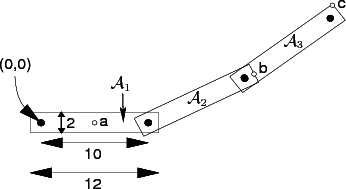
\includegraphics[height=1.5in]{img986}
}
\end{figure}

\textbf{Question: } Consider the articulated chain of bodies shown in Figure 3.29. There are three identical rectangular bars in the plane, called  $ {\cal A}_1,{\cal A}_2,{\cal A}_3$. Each bar has width 2 and length 12. The distance between the two points of attachment is 10. The first bar,  $ {\cal A}_1$, is attached to the origin. The second bar,  $ {\cal A}_2$, is attached to  $ {\cal A}_1$, and  $ {\cal A}_3$ is attached to  $ {\cal A}_2$. Each bar is allowed to rotate about its point of attachment. The configuration of the chain can be expressed with three angles,  $ (\theta_1,\theta_2,\theta_3)$. The first angle, $ \theta_1$, represents the angle between the segment drawn between the two points of attachment of  $ {\cal A}_1$ and the $ x$-axis. The second angle, $ \theta_2$, represents the angle between  $ {\cal A}_2$ and  $ {\cal A}_1$ ( $ \theta_2
= 0$ when they are parallel). The third angle, $ \theta_3$, represents the angle between  $ {\cal A}_3$ and  $ {\cal A}_2$. Suppose the configuration is  $ (\pi/4,\pi/2,-\pi/4)$.
\begin{enumerate}
\item Use the homogeneous transformation matrices to determine the locations of points $ a$, $ b$, and $ c$.

\textbf{Answer: }\begin{align*}
a &= \begin{bmatrix}
\cos(\theta_1) & -\sin(\theta_1) & 0 \\
\sin(\theta_1) &  \cos(\theta_1) & 0 \\
0 & 0 & 1
\end{bmatrix} \begin{pmatrix}
a_x \\
a_y \\
1
\end{pmatrix} = \begin{pmatrix}
5\cos(\pi/4) \\
5\sin(\pi/4) \\
1
\end{pmatrix} = \begin{pmatrix}
5/\sqrt{2} \\
5/\sqrt{2} \\
1
\end{pmatrix} \\
\\
b &= \begin{bmatrix}
C(\theta_1) & -S(\theta_1) & 0 \\
S(\theta_1) &  C(\theta_1) & 0 \\
0 & 0 & 1
\end{bmatrix} \begin{bmatrix}
C(\theta_2) & -S(\theta_2) & x_{01} \\
S(\theta_2) &  C(\theta_2) & y_{01} \\
0 & 0 & 1
\end{bmatrix} \begin{pmatrix}
b_x \\
b_y \\
1
\end{pmatrix} \\
&= \begin{bmatrix}
C_{12} & -S_{12} & x_{01}C_1-y_{01}S_1 \\
S_{12} &  C_{12} & x_{01}S_1+y_{01}C_1 \\
0 & 0 & 1
\end{bmatrix} \begin{pmatrix}
b_x \\
b_y \\
1
\end{pmatrix} = \begin{pmatrix}
-1/\sqrt{2} \\
21/\sqrt{2} \\ 
1
\end{pmatrix} \\
\\
c &= \begin{bmatrix}
C_{12} & -S_{12} & x_{01}C_1-y_{01}S_1 \\
S_{12} &  C_{12} & x_{01}S_1+y_{01}C_1 \\
0 & 0 & 1
\end{bmatrix} \begin{bmatrix}
C_{3} & -S_{3} & x_{12} \\
S_{3} &  C_{3} & y_{12} \\
0 & 0 & 1
\end{bmatrix} \begin{pmatrix}
c_x \\
c_y \\
1
\end{pmatrix} \\
&= \begin{bmatrix}
C_{123} & -S_{123}  &  x_{01}C_1 - y_{01}S_1 + x_{12}C_{12} - y_{12}S_{12} \\
S_{123} &  C_{123}  &  x_{01}S_1 + y_{01}C_1 + x_{12}S_{12} + y_{12}C_{12} \\
0 & 0 & 1
\end{bmatrix} \begin{pmatrix}
c_x \\
c_y \\
1
\end{pmatrix} \\
&= \begin{pmatrix}
-1 \\
20/\sqrt{2} + 10 \\ 
1
\end{pmatrix}
\end{align*}

\item Characterize the set of all configurations for which the final point of attachment (near the end of  $ {\cal A}_3$) is at $ (0,0)$ (you should be able to figure this out without using the matrices).

\textbf{Answer: } 
The points ${\cal A}_0$ and ${\cal A}_3$ are coincident when the three links form a triangle. At that point, the first rotation about the origin will not affect the coincidence. 
Following the law of sines, this coincidence will occur when the following equation holds.
\begin{equation*}
\sin\theta_2 = a_3 \left( \frac{\sin\theta_3}{a_1} \right)
\end{equation*}
For the linkage with all lengths $a_1, a_2, a_3 = 10$, the joint angles $\theta_2$ and $\theta_3$ will be equal to $\pi/3$.
\end{enumerate}


\section{Problem 5.5}
\textbf{Question: } The dispersion definition given in (5.19) is based on the worst case. Consider defining the average dispersion:
\begin{equation}
\bar{\delta}(P) = \frac{1}{\mu(X)} \int_X \min_{p \in P} \{ \rho(x,p) \} dx 
\end{equation}
Describe a Monte Carlo (randomized) method to approximately evaluate the above equation.

\textbf{Answer: } In order to approximate the average dispersion, $\bar{\delta}$, begin by randomly selecting samples, $p$, from the whole set of samples, $P$. For each sample, simply calculate the distance to the nearest neighbor, $\min_{p \in P} \{ \rho(x,p) \}$. This calculation is made simple by cleverly organizing the data structure containing the samples, such as a KD-Tree. Finally, simply average the distances together, yielding the following approximation of the average dispersion, $\bar{\delta}$. 
\begin{equation}
\hat{\delta} = \frac{1}{n}\sum^{n}_{i=0} \min_{p \in P} \{ \rho(x_{rand},p) \}
\end{equation}


\section{Problem 5.15}
\textbf{Question: } Design combinations of robots and obstacles in $ {\cal W}$ that lead to C-space obstacles resembling bug traps.

\textbf{Answer: } Any robot with sufficiently complex shape (Can not be reliably approximated as a cylinder in 3D or circle in 2D), and with a narrow passage exiting a room with only one door will create a "bug trap" shape. This is especially if this door is far from the robot and not visible from the starting configuration. 

For a kinematic chain (i.e. a robot arm), attempting to reach down a long tube will also create a "bug trap" in C space. This is especially true if the tube is thin-walled, allowing the robot arm to move freely around it. 




\section{Problem 5.17}
\textbf{Question: } In a high-dimensional grid, it becomes too costly to consider all $ 3^n-1$ $ n$-neighbors. It might not be enough to consider only $ 2n$ 1-neighbors. Determine a scheme for selecting neighbors that are spatially distributed in a good way, but without requiring too many. For example, what is a good way to select $ 50$ neighbors for a grid in  $ {\mathbb{R}}^{10}$?

\textbf{Answer: } The most important characteristic of a neighborhood is that it provides coverage of the entire space. In order to guarantee this, it is good to always include the 2 singly-connected neighbors for each axis (positive and negative step along axis). This accounts for the first $2n$ neighbors, or 20 in $\mathbb{R}^{10}$. 

With these base neighbors, the entire C-space is now reachable through neighbor relationships. At this point, the remaining number of neighbors should be selected, maximizing the distance between them. 
\begin{equation}
\operatorname*{arg\,max}_P \left\lbrace 	\sup_{x \in X} \big\{ \min_{p \in P} \big\{ \rho(x,p) \big\}\big\}. \right\rbrace
\end{equation}


\section{Problem 5.18}
\textbf{Question: } Explain the difference between searching an implicit, high-resolution grid and growing search trees directly on the C-space without a grid.

\textbf{Answer: } Searching directly on the C-space without a grid allows the algorithm to approach the goal configuration exactly, by periodically selecting the goal, $q_{goal}$, rather than some random $q$ value. 

A grid would require an arbitrarily small grid to achieve the same result, making the search painstakingly slow. 

\pagebreak
\section{Implementation}
\subsection{1.1 Superior 4-Connected Heuristic}
Of the two 4-connected paths generated above, the path generated using the Manhattan heuristic appears to be the best. Since the robot is always traveling on the vertical or horizontal axes, the two paths are the same length. However, the Manhattan heuristic path is superior, because it requires far fewer changes in direction. When executing, the robot will be able to traverse this path much faster, as it does not need to stop and change direction every few inches. 
\subsection{1.2 Superior 8-Connected Heuristic}
For the 8-connected paths, however, the Euclidian metric appears superior. The two paths in this case are \emph{not} the same length. The Euclidian path is much shorter, as it makes use of the diagonal paths as often as possible. 
\subsection{1.3 Admissible and Inadmissible Heuristics}
All of the paths generated above are admissible, because they use identical metrics for both heuristic and cost evaluation. 


\begin{figure}
\centerline{\begin{subfigure}{.6\textwidth}
  \centering
  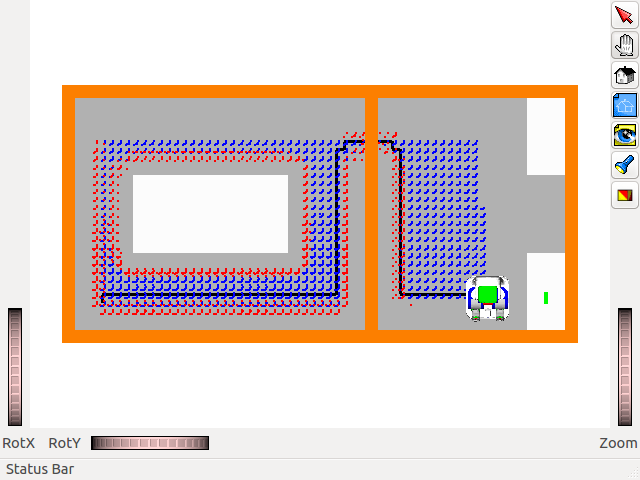
\includegraphics[width=.9\linewidth]{../Screenshots/4-Manhattan}
  \caption{4-Connected Manhattan}
  \label{fig:4Man}
\end{subfigure}%
\begin{subfigure}{.6\textwidth}
  \centering
  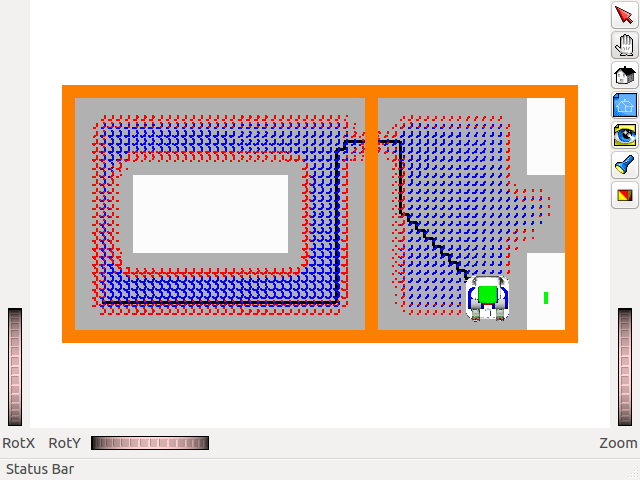
\includegraphics[width=.9\linewidth]{../Screenshots/4-Euclidian}
  \caption{4-Connected Euclidian}
  \label{fig:4Euc}
\end{subfigure}}
\centerline{\begin{subfigure}{.6\textwidth}
  \centering
  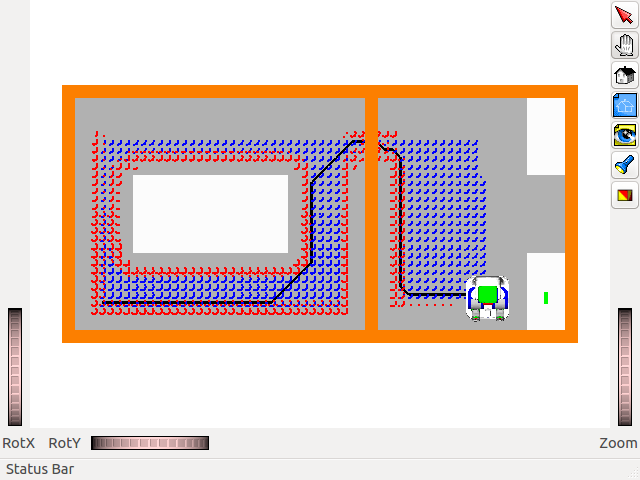
\includegraphics[width=.9\linewidth]{../Screenshots/8-Manhattan}
  \caption{8-Connected Manhattan}
  \label{fig:8Man}
\end{subfigure}%
\begin{subfigure}{.6\textwidth}
  \centering
  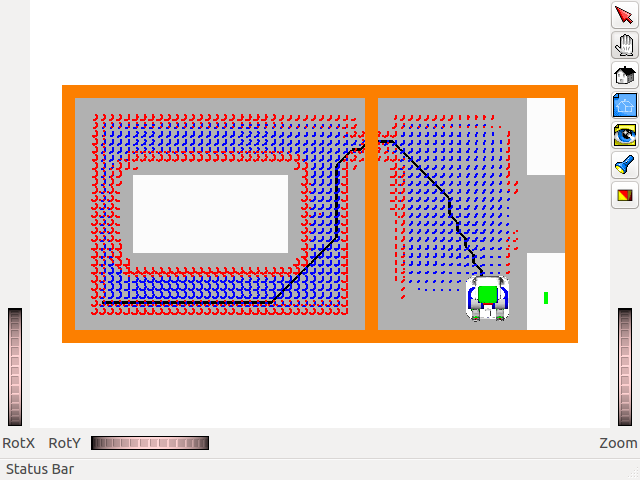
\includegraphics[width=.9\linewidth]{../Screenshots/8-Euclidian}
  \caption{8-Connected Euclidian}
  \label{fig:8Euc}
\end{subfigure}}
\caption{Paths found by A* algorithm with varying connectedness and distance metrics}
\label{fig:fig}
\end{figure}

\end{document}



